\section{Numerical Part}
%

We will now study numerically the Hamiltonian (\ref{eq2.1}) and we will compare the numerical with the analytical results. In order to do that, we will construct its Poincare Map. In order to do so, we will have to solve numerically the following Hamilton's equations of motion
	\begin{align*}
	\left\{
		\begin{matrix}
			\dot{\theta} =& \pdv{H}{J     }  \vspace{0.3cm}\\
			\dot{J     } =& -\pdv{H}{\theta}
		\end{matrix}  \right. \Rightarrow \\
	\end{align*}\vspace{-1.2cm}
	\begin{align*}
		\left\{
		\begin{matrix}
			\dot{\theta} =& \bar{\omega} + kJ^{k-1} \\
			\dot{J     } =& V_1n_1sin(n_1\theta-m_1\Omega t) + V_2n_2sin(n_2\theta-m_2\Omega t)
		\end{matrix}  \right.
	\end{align*}
	We choose $\Omega=1$, $\bar{\omega}=1$, $k=2$,\footnote{As we increase k, $\Delta J_{res,1,2}=|\Delta J_{res,1}-\Delta J_{res,2}|$, becomes smaller and smaller. So, in order to maintain a clear plot in which the resonace island wont overlap even for small $V_1,V_2$ vales, we choose $k=2$}
	and $n_1=3,m_1=6,n_2=4,m_2=6$ depending on which combination gives a cool final diagram( :) )\footnote{We may observe that the number of resonance islands is equal to $n_i$, so if we choose $n_1=3,n_2=4$, we will have 3 resonance islands for the perturbation 1 and 4 for the perturbation 2.}.
	The expected resonance \textit{Actions} from (\ref{eq2.7}) are 
		\begin{align*}
			J_{res,1} = & 0.5\\ 
			J_{res,2} = & 0.25 
		\end{align*}
		%
	If we set the perturbations, $V_1,V_2=0$, we obtain a Poincare diagram where the \textit{Action} is constant of motion, since the Hamiltonian $H_1$ is integrable. This is shown in (\ref{fig2.1})
	\begin{figure}[h!]
		\centering
		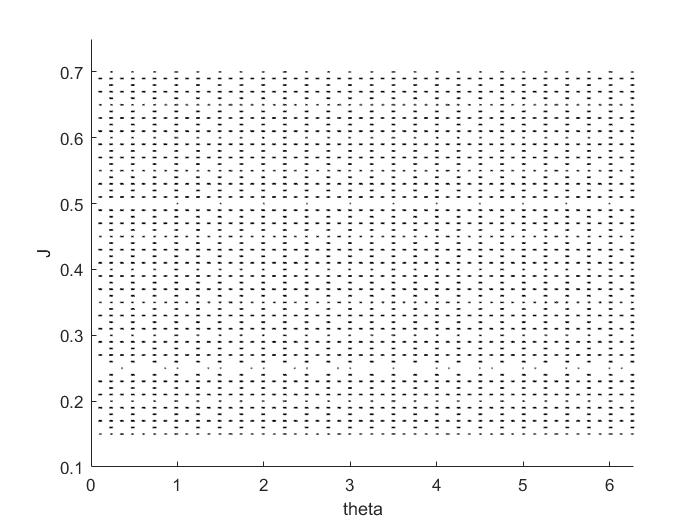
\includegraphics[scale=0.5]{Hamiltonian_1/numerical/figs/Q5_0.0_3646}
		\caption{$V_1=0,V_2=0$ and we see that J is a constant of motion.}
		\label{fig2.1}	
	\end{figure}\newpage
%
%
Now, we increase control values of the perturbations to $V_1=V_2=10^{-4}$ and we obtain (\ref{fig2.2}) \footnote{The different colors correspond to different initial conditions for $\theta$.}
	\begin{figure}[h!]
		\centering 
		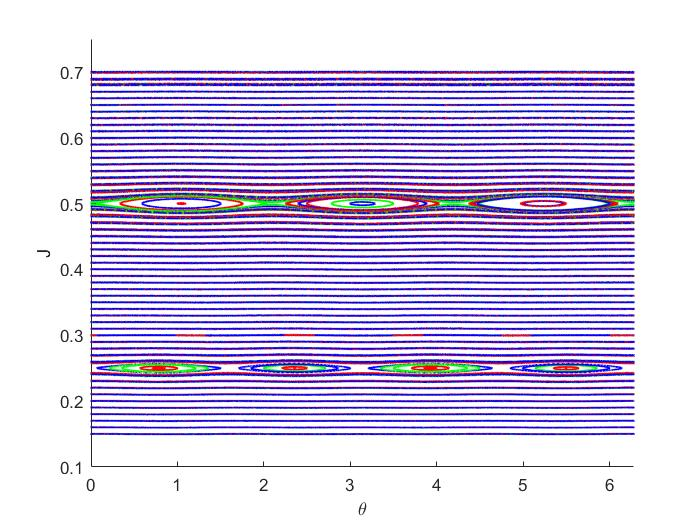
\includegraphics[scale=0.5]{Hamiltonian_1/numerical/figs/Q5_1e-4.1e-4_3634}
		\caption{$V_1=V_2=10^{-4}$ we see that the resonance island emerge at the theoretically expected values of Action}
		\label{fig2.2}
	\end{figure}\\
	
If we further increase the perturbations to $V_1=10^{-3},V_2=10^{-4}$ and $V_1=10^{-4},V_2=10^{-3}$ we have (Figure \ref{fig2.3}), where we see that the islands that correspond to the bigger $V_i$ are larger.\\
%
\begin{figure}[h!]
	\centering
	\begin{subfigure}{.5\textwidth}
  		%\centering
  		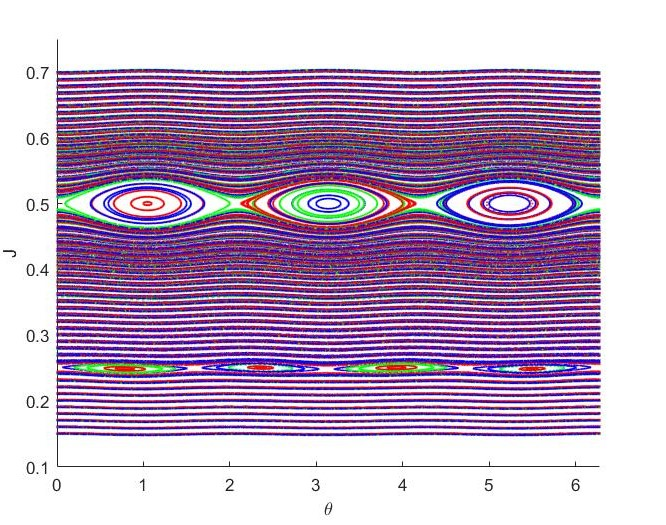
\includegraphics[scale=0.5,left]{Hamiltonian_1/numerical/figs/Q5_1e-3.1e-4_3634}
  		\caption{$V_1=10^{-3},V_2=10^{-4}$}
  		\label{fig2.3a}
	\end{subfigure}%
	\begin{subfigure}{.5\textwidth}
  		%\centering
  		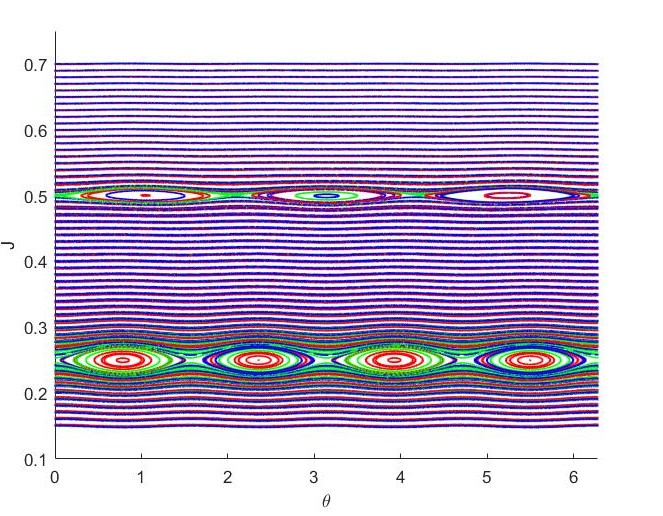
\includegraphics[scale=0.5,right]{Hamiltonian_1/numerical/figs/Q5_1e-4.1e-3_3634}
  		\caption{$V_1=10^{-4},V_2=10^{-3}$}
  		\label{fig2.3b}
	\end{subfigure}
	\caption{Larger $V_i$ corresponds to larger resonance island.}
	\label{fig2.3}
\end{figure}
	%
\begin{figure}[h!]
	\centering
	\begin{subfigure}{.5\textwidth}
  		%\centering
  		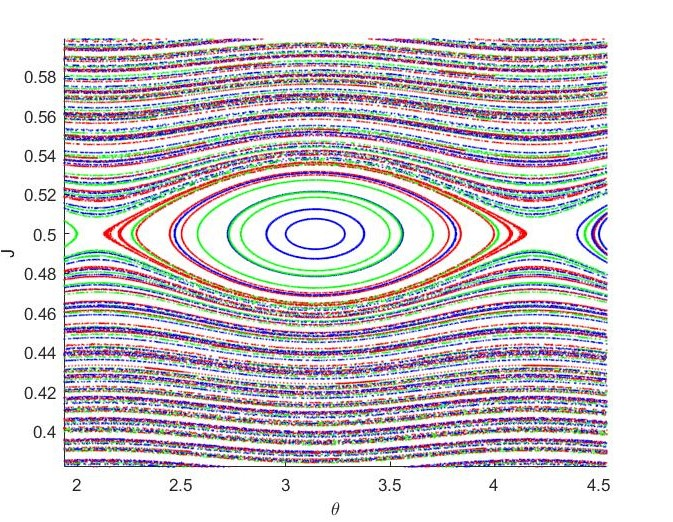
\includegraphics[scale=0.5,left]{Hamiltonian_1/numerical/figs/Q5_1e-3.1e-4_3634_zoom}
  		\caption{$V_1=10^{-3},V_2=10^{-4}$, upper-large islands}
  		\label{fig2.4a}
	\end{subfigure}%
	\begin{subfigure}{.5\textwidth}
  		%\centering
  		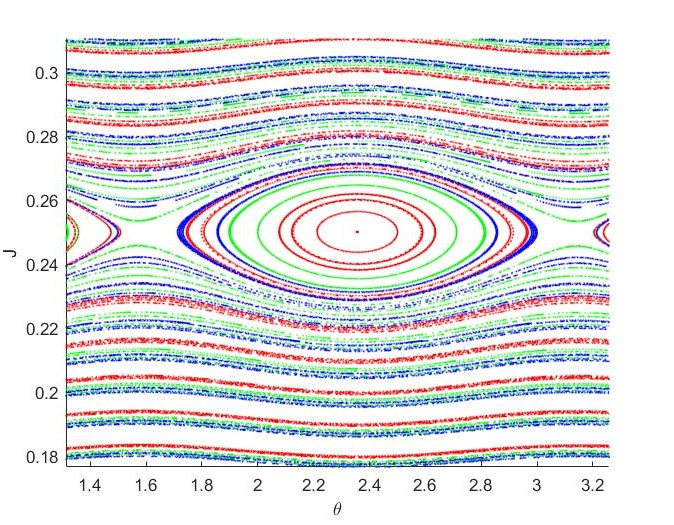
\includegraphics[scale=0.5,right]{Hamiltonian_1/numerical/figs/Q5_1e-4.1e-3_3634_zoom}
  		\caption{$V_1=10^{-4},V_2=10^{-3}$, lower-large islands}
  		\label{fig2.4b}
	\end{subfigure}
	\caption{(Zoomed (Figure \ref{fig2.3})) We see that the islands that correspond to the larger perturbation also have the same width $\Delta J\simeq 0.04$}
	\label{fig2.4}
\end{figure}	\newpage
%
As we increase the value of the perturbations to $V_1=V_2=10^{-3}$ the islands grow larger 
	\begin{figure}[h!]
		\centering
		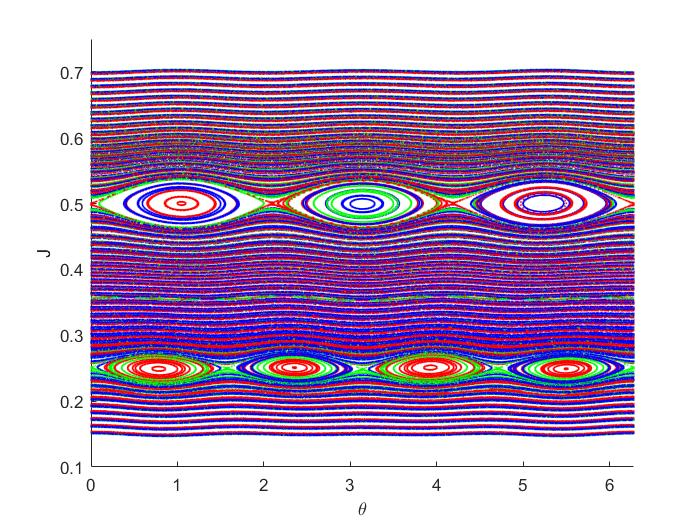
\includegraphics[scale=0.5]{Hamiltonian_1/numerical/figs/Q5_1e-3.1e-3_3634}
		\label{fig2.5}
		\caption{$V_1=V_2=10^{-3}$}
	\end{figure}\\
	%
	Now if we set $V_1=10^{-2}, V_2=10^{-3}$ and $V_1=10^{-3},V_2=10^{-2}$, we see in (Figure (\ref{fig2.6}) that the phase space around the larger perturbation is heavily distorted. 
	%
\begin{figure}[H]
	\centering
	\begin{subfigure}{.5\textwidth}
  		\centering
  		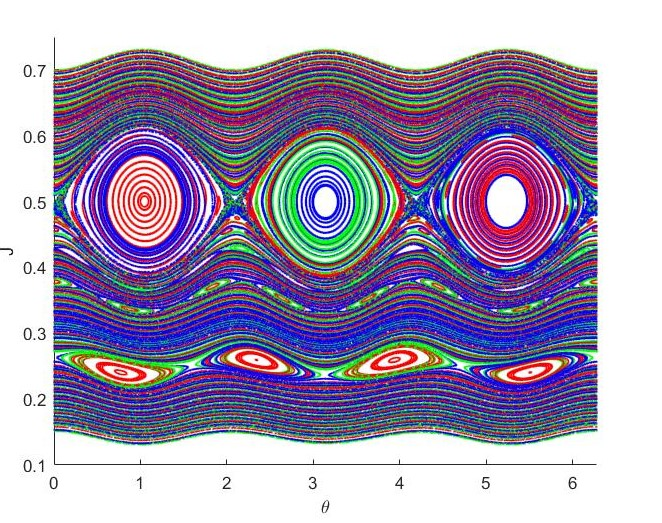
\includegraphics[scale=0.5,left]{Hamiltonian_1/numerical/figs/Q5_1e-2.1e-3_3634}
  		\caption{$V_1=10^{-2},V_2=10^{-3}$, upper-large islands}
  		\label{fig2.6a}
	\end{subfigure}%
	\begin{subfigure}{.5\textwidth}
  		%\centering
  		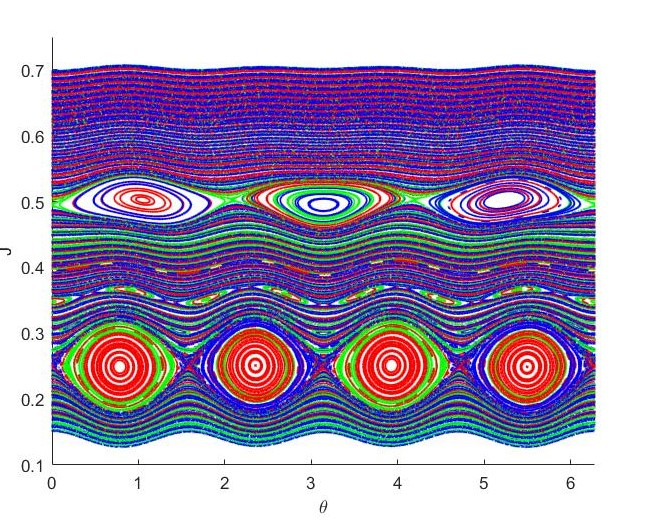
\includegraphics[scale=0.5,right]{Hamiltonian_1/numerical/figs/Q5_1e-3.1e-2_3634}
  		\caption{$V_1=10^{-3},V_2=10^{-2}$, lower-large islands}
  		\label{fig2.6b}
	\end{subfigure}
	\caption{ Again we see that bigger $V_i$ corresponds to larger islands}
	\label{fig2.6}
\end{figure}
%
%zoomed 2.6
\begin{figure}[H]
	\centering
	\begin{subfigure}{.5\textwidth}
  		%\centering
  		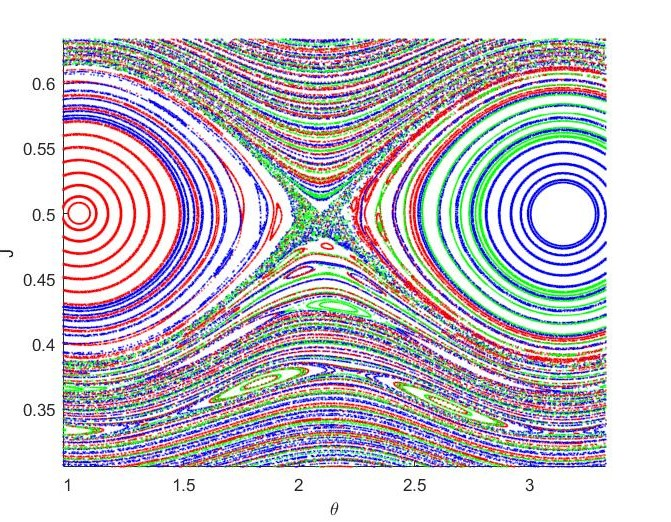
\includegraphics[scale=0.47,left]{Hamiltonian_1/numerical/figs/Q5_1e-2.1e-3_3634_zoom1}
  		\caption{$V_1=10^{-2},V_2=10^{-3}$, upper-large islands}
  		\label{fig2.7a}
	\end{subfigure}%
	\begin{subfigure}{.5\textwidth}
  		%\centering
  		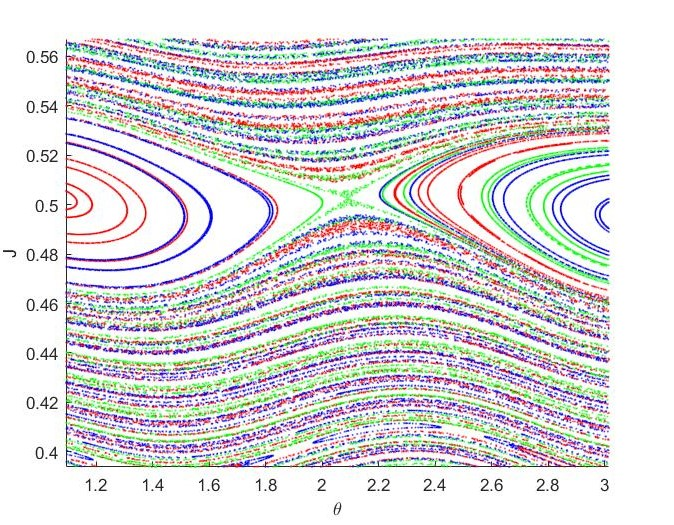
\includegraphics[scale=0.47,right]{Hamiltonian_1/numerical/figs/Q5_1e-3.1e-2_3634_zoom1}
  		\caption{$V_1=10^{-3},V_2=10^{-2}$, lower-large islands}
  		\label{fig2.7b}
	\end{subfigure}
	        %\vskip\baselineskip
	\begin{subfigure}{.49\textwidth}
  		%\centering
  		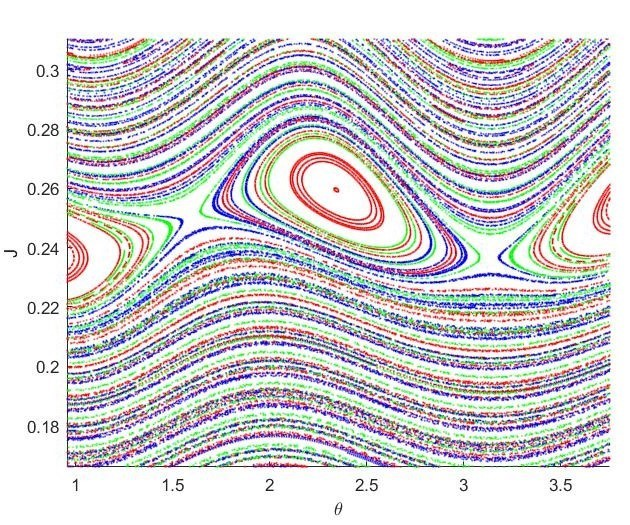
\includegraphics[scale=0.47,left]{Hamiltonian_1/numerical/figs/Q5_1e-2.1e-3_3634_zoom2}
  		\caption{$V_1=10^{-3},V_2=10^{-2}$, lower-large islands}
  		\label{fig2.7c}
	\end{subfigure}
	\begin{subfigure}{.49\textwidth}
  		%\centering
  		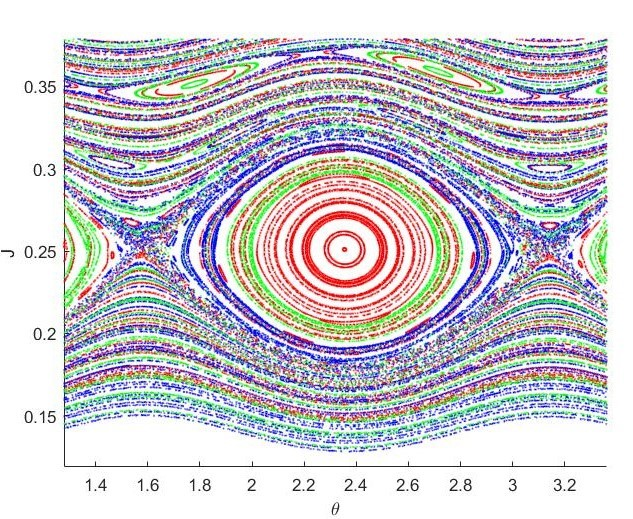
\includegraphics[scale=0.47,right]{Hamiltonian_1/numerical/figs/Q5_1e-3.1e-2_3634_zoom2}
  		\caption{$V_1=10^{-3},V_2=10^{-2}$, lower-large islands}
  		\label{fig2.7d}
	\end{subfigure}
	\caption{(Zoomed (Figure \ref{fig2.6})) We see that the islands that correspond to the larger perturbation also have the same width $\Delta J\simeq 0.04$}
	\label{fig2.7}
\end{figure}
Now, we set both $V_1=V_2=10^{-2}$ and we have (Figure \ref{fig2.8}). As we seem the two separatrices overlap and we have extended chaos.
%
\begin{figure}[H]
	\centering
	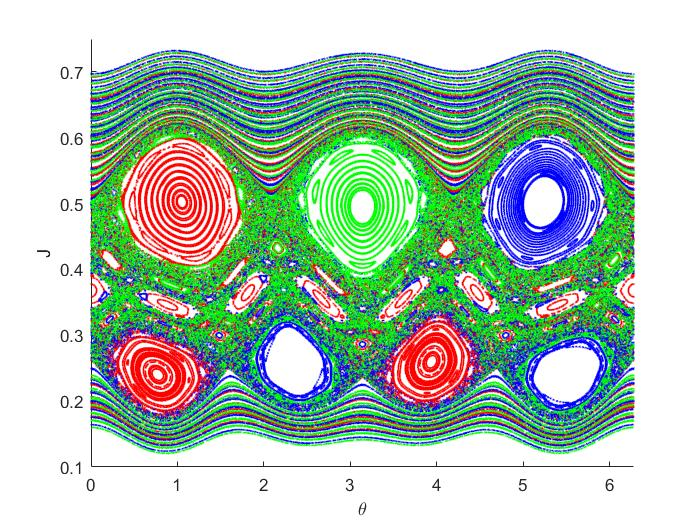
\includegraphics[scale=0.6]{Hamiltonian_1/numerical/figs/Q5_1e-2.1e-2_3634}
	\caption{$V_1=V_2=10^{-2}$}
	\label{fig2.8}
\end{figure}
%x
\begin{figure}[H]
	\centering
	\begin{subfigure}{.32\textwidth}
  		\centering
  		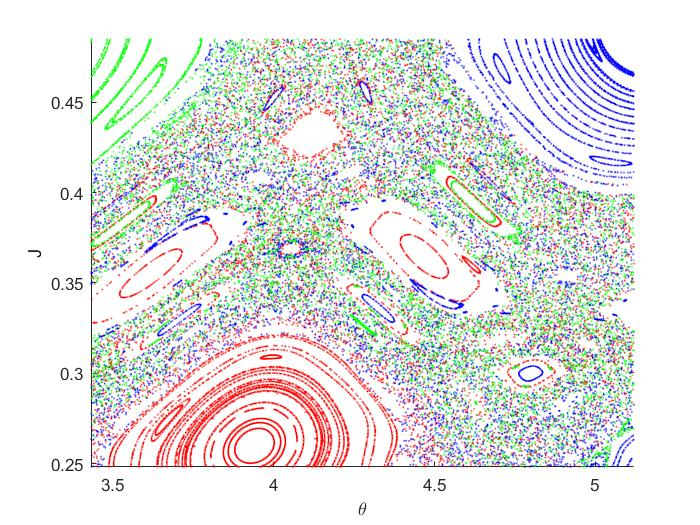
\includegraphics[scale=0.25]{Hamiltonian_1/numerical/figs/Q5_1e-2.1e-2_3634_zoom1}
  		%\caption{$V_1=10^{-2},V_2=10^{-2}$, upper-large islands}
  		\caption{}
  		\label{fig2.9a}
	\end{subfigure}%
	\begin{subfigure}{.32\textwidth}
  		\centering
  		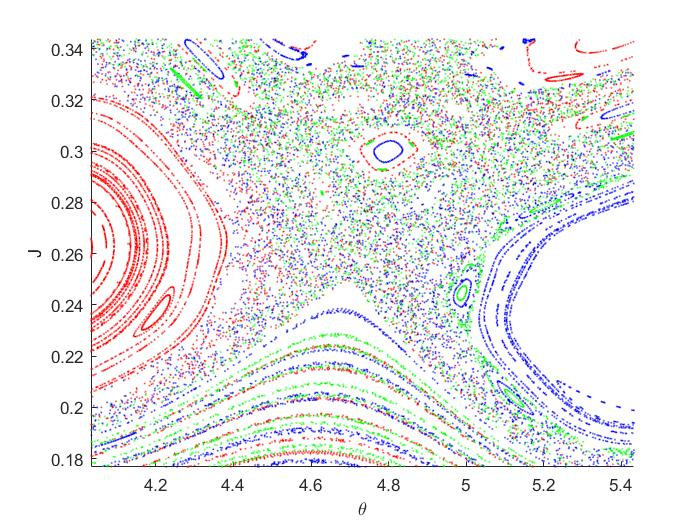
\includegraphics[scale=0.25]{Hamiltonian_1/numerical/figs/Q5_1e-2.1e-2_3634_zoom2}
  		%\caption{$V_1=10^{-2},V_2=10^{-2}$, lower-large islands}
  		\caption{}
  		\label{fig2.9b}
	\end{subfigure}
	%
	\begin{subfigure}{.32\textwidth}
		\centering
		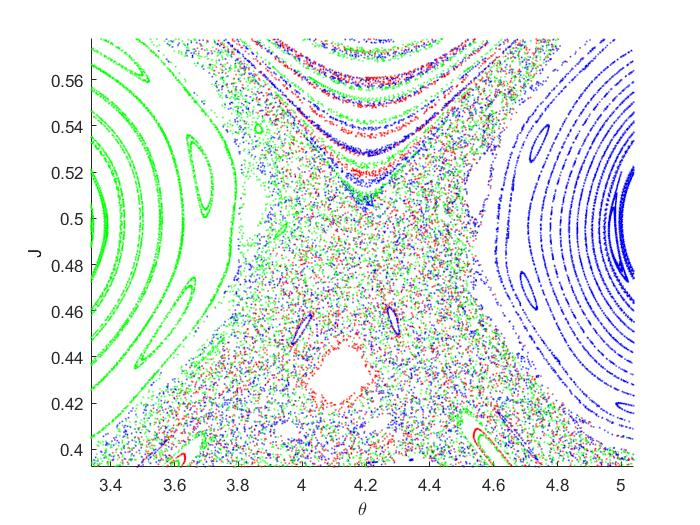
\includegraphics[scale=0.25]{Hamiltonian_1/numerical/figs/Q5_1e-2.1e-2_3634_zoom3}
		\caption{}
		\label{fig2.9c}
	\end{subfigure}
	\label{fig2.9}
	\caption{Zoom in (Figure \ref{fig2.8})}
\end{figure}
%
%%

We can make another remark on the above diagrams. From [1], we have that the width of the resonance islands, that is the distance between the two separatrices, is given by the relation 
	\begin{align*}\label{eq2.22}
		\Delta J_{i,max}= 2n_i \left( \frac{2V_i}{G}\right)^{1/2}
	\end{align*}
	where $G=n_i^2\partial^2(H_0)/\partial^2(J_i)$.
So, for various values of $V_1,V_2$, we have the following values 
\newpage
	\begin{table}[th]
		\centering 
		\begin{tabular}{c|c||c|c}
			$V_1$ & $\Delta J_{1,max}$ & $V_2$ & $\Delta J_{2,max}$ \\ 
			\hline\hline
			$10^{-4}$ & 0.0200& $10^{-4}$ & 0.0200 \\ 
			$10^{-3}$ & 0.0632& $10^{-3}$ & 0.0632 \\
			$10^{-2}$ & 0.2000& $10^{-2}$ & 0.2000 
		\end{tabular}
		\caption{}
		\label{tab2.1}
	\end{table}
	We can notice that for $V_1=V_2=10^{-2}$ the resonace islands overlap which is something that we have already found from the numerical results (Figure \ref{fig2.8}).
	In order to compare the above results with the numerical ones, we use the same code as before, but we restrict the Poincare sections only at a fraction of the phase space near the resonances. In that way we can approximate the separatrices and compare their distance with the values of the Table (\ref{tab2.1}).
\begin{figure}[hb!]
	\centering
	\begin{subfigure}{.49\textwidth}
  		%\centering
  		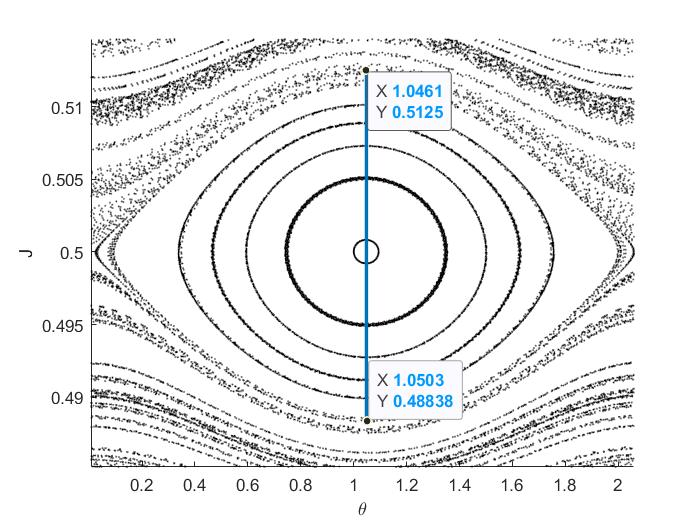
\includegraphics[scale=0.3,left]{Hamiltonian_1/numerical/figs/Q5_dj_1e-4_res1}
  		\caption{$V_1=V_2=10^{-4}$, $J_{res,1}=0.5$ with \\$\Delta J_{1,res}=0.024$}
  		\label{fig2.10a}
	\end{subfigure}%
	\begin{subfigure}{.5\textwidth}
  		%\centering
  		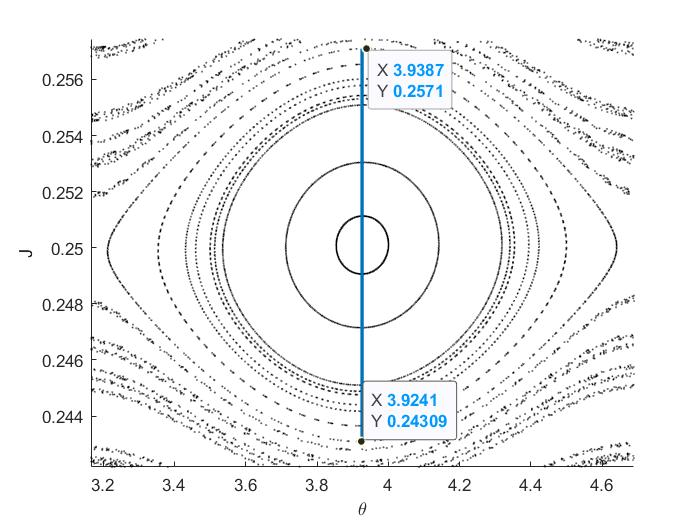
\includegraphics[scale=0.3,right]{Hamiltonian_1/numerical/figs/Q5_dj_1e-4_res2}
  		\caption{$V_1=V_2=10^{-4}$, $J_{res,2}=0.25$ with \\$\Delta J_{2,res}=0.14$}
  		\label{fig2.10b}
	\end{subfigure}%
	        %\vskip\baselineskip
	        \\
	\begin{subfigure}{.49\textwidth}
  		%\centering
  		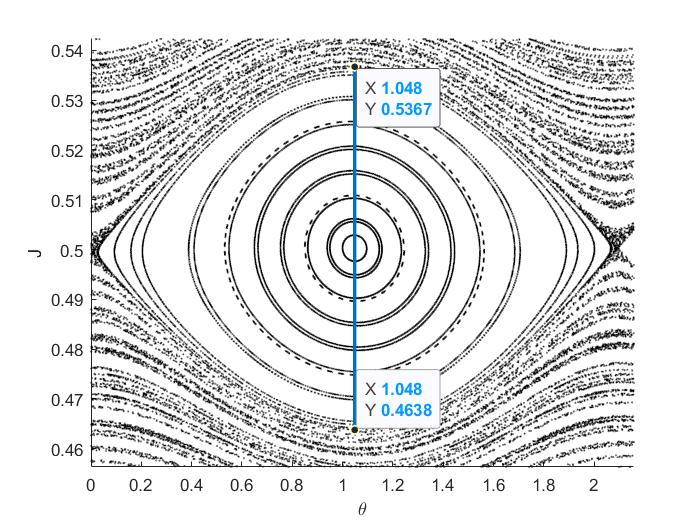
\includegraphics[scale=0.3,left]{Hamiltonian_1/numerical/figs/Q5_dj_1e-3_res1}
  		\caption{$V_1=V_2=10^{-3}$, $J_{res,1}=0.5$ with \\$\Delta J_{1,res}=0.073$}
  		\label{fig2.10c}
	\end{subfigure}
	%
	\begin{subfigure}{.49\textwidth}
  		%\centering
  		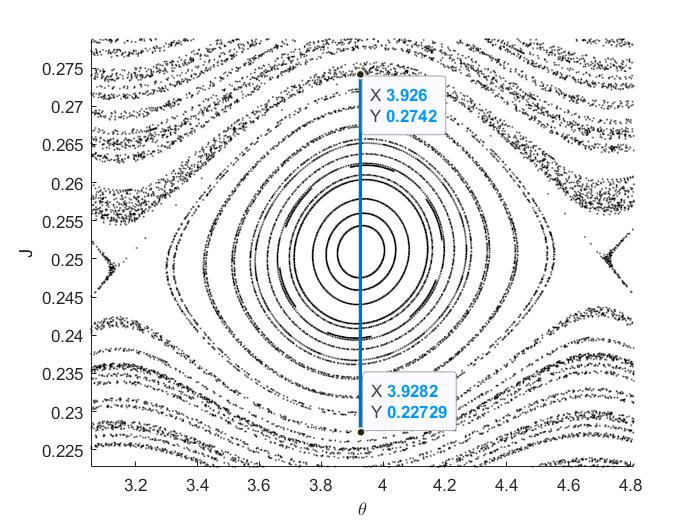
\includegraphics[scale=0.3,right]{Hamiltonian_1/numerical/figs/Q5_dj_1e-3_res2}
  		\caption{$V_1=V_2=10^{-3}$, $J_{res,2}=0.25$ with \\$\Delta J_{2,res}=0.044$}
  		\label{fig2.10d}
	\end{subfigure}	
	%
%	\begin{subfigure}{.49\textwidth}
%  		%\centering
%  		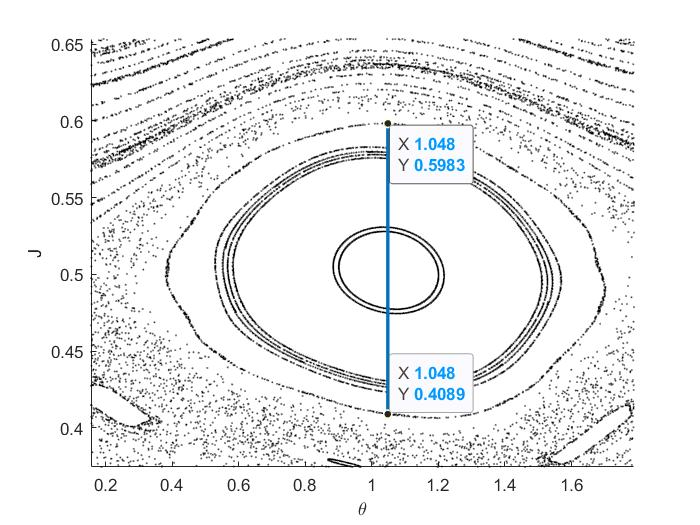
\includegraphics[scale=0.3,left]{Hamiltonian_1/numerical/figs/Q5_dj_1e-2_res1}
%  		\caption{$V_1=V_2=10^{-2}$, $J_{res,1}=0.5$ with $\Delta J_{1,res}=$}
%  		\label{fig2.10e}
%	\end{subfigure}
%	\begin{subfigure}{.49\textwidth}
%  		%\centering
%  		\includegraphics[scale=0.3,right]{Hamiltonian_1/numerical/figs/Q5_dj_1e-2_res2}
%  		\caption{$V_1=V_2=10^{-2}$, $J_{res,2}=0.5$ with $\Delta J_{2,res}=$}
%  		\label{fig2.10f}
%	\end{subfigure}	
	\caption{Poincare Sections to approcimate $\Delta J_{i,res}$ from the numerical results}
	\label{fig2.10}
\end{figure}\\
There analytical and numerical results are relatively close. There are no plots for $V_i=10^{-2}$ since the resonance regions overlap and there are no clear limits of the separatrices.